\documentclass{report}
\usepackage{amsmath}
\usepackage{amsthm}
\usepackage{amsfonts}
\usepackage{mathrsfs}
\usepackage{bm}
\usepackage[usenames,dvipsnames]{xcolor}
\usepackage{tikz}
\usepackage{hyperref}

\hypersetup{
    colorlinks,
    linkcolor={red!30!black},
    citecolor={blue!50!black},
    urlcolor={blue!80!black}
}


\begin{document}



\newcommand{\vct}[1]{\mathbf{#1}}
\newcommand{\vx}{\vct{x}}
\newcommand{\vy}{\vct{y}}
\newcommand{\Z}{\mathcal{Z}}
\newcommand{\E}{\mathcal{E}}
\newcommand{\Ham}{\mathcal{H}}
\newcommand{\W}{\mathcal{W}}
\newcommand{\A}{\mathcal{A}}
\newcommand{\LL}{\mathcal{L}}
\newcommand{\var}{\mathrm{var}}
\newcommand{\com}{\mathrm{com}}

\newcommand{\llbra}{[\![}
\newcommand{\llket}{]\!]}

% annotation macros
\newcommand{\repl}[2]{{\color{gray} [#1] }{\color{blue} #2}}
\newcommand{\add}[1]{{\color{blue} #1}}
\newcommand{\del}[1]{{\color{gray} [#1]}}
\newcommand{\note}[1]{{\color{OliveGreen}\small [\textbf{Comment.} #1]}}





\title{Markov-chain Monte Carlo Simulations}
\author{ \vspace{-10ex} }
\date{ \vspace{-10ex} }


\maketitle

\abstract{
  In this note, we try to explain Markov-chain Monte Carlo simulations work.
  %
  The focus are the properties of a general transition matrix,
  and how they lead to the Perron-Frobenius theorem.
}

%\tableofcontents



\chapter{Transition matrices}



In this chapter, we shall review the basics of
Markov chains and transition matrices
and how they lead to a unique stationary distribution
(Perron-Frobenius theorem).
%
Our main source is Van Kampen\cite{vankampen},
Chapter 5.


\section{Probability distributions
and stochastic processes}



A discrete probability \emph{distribution}
is an array of $N$ numbers
\begin{equation}
  \mathbf p
  =
  (p_1, \dots, p_N),
\end{equation}
with
\begin{equation}
  p_k \ge 0,
  \qquad
  \mathrm{and}
  \qquad
  \sum_{ k = 1 }^N p_k = 1.
\label{eq:probreq}
\end{equation}

In a \emph{stochastic process},
the distribution $\mathbf p(t)$
changes with time $t$.


Now there are at least two ways of
interpreting probability.
%
\begin{enumerate}
  \item
  The frequency way:
  if I roll a dice many times,
  the frequency of me getting the number $i$
  is given by $p_i$.

  \item
  The population or ensemble way:
  if there are $10^6$ people like me,
  and everyone of them rolls a dice;
  then there are roughly $10^6 \times p_i$ of them
  getting the number $i$.

\end{enumerate}


The first way is rather clumsy
for studying stochastic processes.
%
This is because by interpreting probabilities as
frequencies, we have to image, at any given time $t$,
a \emph{repeated} experiment, which demands
another time dimension.
%
But imagining two time dimensions
can be quite stressful to the brain.
%
On the other hand,
we can think readily imagine at any time
there are $10^6$ people standing
on $N$ different sites.
Then they start to move about
among the sites as $t$ changes.
%
This makes the population interpretation
more convenient.



\section{Markov chain}




A \emph{Markov process} is special stochastic process,
in which the system has no memory.
%
Assuming discrete time, then
the distribution $\mathbf p(t+1)$ at time $t + 1$
depends only on distribution
$\mathbf p(t)$ at the previous time, $t$.
%
Usually we assume that the dependence is linear, so that
$$
  \mathbf p(t+1)
  =
  \mathbf T(t) \, \mathbf p(t). 
$$
where $\mathbf T(t)$ is a $N$ by $N$ square matrix.
%
If $\mathbf T(t)$ is independent of time,
then we call this process a \emph{Markov chain}.
%
The time evolution of the probability follows
%
\begin{equation}
  \mathbf p(t+1)
  =
  \mathbf T \, \mathbf p(t),
\label{eq:mcp}
\end{equation}
%
and $\mathbf T$ is the transition matrix.


Now Eq. \eqref{eq:mcp} is a matrix equation.
In practice, we always need to write it in component form
%
\begin{equation}
  p_i(t + 1)
  =
  T_{i1} \, p_1(t)
  + \cdots +
  T_{iN} \, p_N(t)
  =
  \sum_{j = 1}^N T_{ij} \, p_j(t)
  .
\end{equation}
%
We can represent the components $T_{ij}$
graphically as follows:
%
\begin{figure}[h]
  \centering
  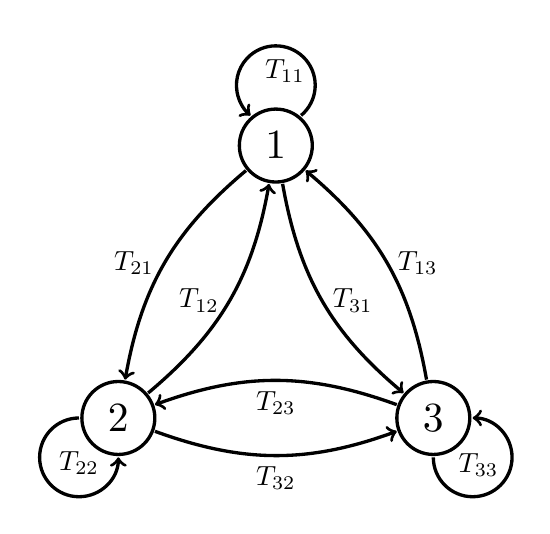
\begin{tikzpicture}
    \node[draw, circle, very thick, scale=1.5] (1) at (2, 3.46) {$1$};
    \node[draw, circle, very thick, scale=1.5] (2) at (0, 0)    {$2$};
    \node[draw, circle, very thick, scale=1.5] (3) at (4, 0)    {$3$};
    \draw[->, very thick]
        (1) edge[bend right=20] node [left]   {$T_{21}$} (2)
        (2) edge[bend right=20] node [below]  {$T_{32}$} (3)
        (3) edge[bend right=20] node [right]  {$T_{13}$} (1)
        (1) edge[bend right=20] node [right]  {$T_{31}$} (3)
        (2) edge[bend right=20] node [left]   {$T_{12}$} (1)
        (3) edge[bend right=20] node [below]  {$T_{23}$} (2)
        ;
    % self arrows
    % ++(50:5mm) shift the start point to node 1 + 5mm * (cos(50), sin(50))
    \draw [->, very thick] (1) ++(50:5mm)
        node [anchor=-70, inner sep=4mm] {$T_{11}$}
        arc (-50:230:5mm);
    % ++(180:5mm) shift the start point to node 2 + (-5mm, 0)
    \draw [->, very thick] (2) ++(180:5mm)
        node [anchor=90, inner sep=4mm] {$T_{22}$}
        arc (-270:0:5mm); 
    \draw [->, very thick] (3) ++(-90:5mm)
        node [anchor=170, inner sep=3mm] {$T_{33}$}
        arc (-180:90:5mm);
  \end{tikzpicture}
\end{figure}



\section{Transition matrix}


The transition matrix

\bibliographystyle{plain}
\bibliography{simul}

\end{document}
